\subsection{Dihedral angle}

\begin{figure}[H]
    \centering
    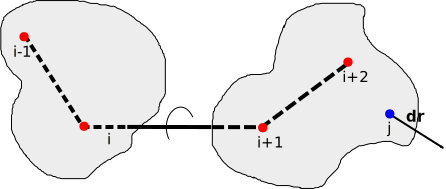
\includegraphics[width=\linewidth]{Fig/DihedralKinematics.png}
    \caption{The model of dihedral angle change upon changing an an atom coordinate.}
    \label{Fig:DihedralKinematics}
\end{figure}

Here, the derivation for the points in two bodies that do not lie on the line $i, i+1$ is essentially the same. Except
we already have a fixed rotation axis $\mathbf{w} = \frac{\mathbf{r}_{i+1} - \mathbf{r}_i}{|\mathbf{w}|}$, which is 
negative for the left body and positive for the right one.
The movement of point $i$ and $i+1$ requires special treatment deserves: in this case the rotation axis moves itself.
The angle of rotation can be computed as follows:
$$
\beta = \arccos \left( \frac{ \left([\mathbf{u}, \mathbf{w}], [\mathbf{w}, \mathbf{v}] \right) }{\sin(\alpha_{i-1}) \sin(\alpha_{i})} \right)
$$
In this case I took the expressions from MODELLER \cite{}:
$$
\begin{array}{lcl}
\frac{d\beta_i}{dr_{i}} &=& -\frac{1}{\sin(\beta)} \left( [\mathbf{r}_{i,i+1}, \mathbf{a}] - [\mathbf{r}_{i+1,i+2}, \mathbf{b}] \right) \\
\frac{d\beta_i}{dr_{i+1}} &=& -\frac{1}{\sin(\beta)} \left( [\mathbf{r}_{i,i+2}, \mathbf{b}] - [\mathbf{r}_{i-1,i}, \mathbf{a}] \right) \\
\mathbf{a} &=& \frac{1}{\left| [\mathbf{r}_{i-1,i}, \mathbf{r}_{i+1,i+2}] \right|} 
    \left( 
        \frac{[\mathbf{r}_{i+1,i}, \mathbf{r}_{i+1,i+2}]}{\left| [\mathbf{r}_{i+1,i}, \mathbf{r}_{r+1,i+2}] \right|} - 
        \cos(\beta)
        \frac{[\mathbf{r}_{i-1,i}, \mathbf{r}_{i+1,i+2}]}{\left| [\mathbf{r}_{i-1,i}, \mathbf{r}_{r+1,i+2}] \right|}
    \right)\\

\mathbf{b} &=& \frac{1}{\left| [\mathbf{r}_{i+1,i}, \mathbf{r}_{i+1,i+2}] \right|} 
    \left( 
        \frac{[\mathbf{r}_{i-1,i}, \mathbf{r}_{i+1,i}]}{\left| [\mathbf{r}_{i-1,i}, \mathbf{r}_{r+1,i}] \right|} - 
        \cos(\beta)
        \frac{[\mathbf{r}_{i+1,i}, \mathbf{r}_{i+1,i+2}]}{\left| [\mathbf{r}_{i+1,i}, \mathbf{r}_{r+1,i+2}] \right|}
    \right)
\end{array}
$$

\begin{algorithm}
    \caption{Bending matrix computation}
    \label{alg:BendingAlgorithm}
    \begin{algorithmic}
        \FOR {$i = 0 \dots N$ scanning bending angles} 
            \FOR {$j = 0 \dots N+2$ scanning atoms} 
                \IF {$j < i $ (atom in left body)}
                    \STATE $\mathbf{\widetilde{r}} = \mathbf{r}_j - \mathbf{r}_{i}$
                    \STATE $\mathbf{w} = \frac{[\mathbf{r}_{i+1} - \mathbf{r}_{i}]}{|\mathbf{w}|}$
                    \STATE $\frac{d\beta_i^k}{dr^k_j} = \frac{[\mathbf{w},\mathbf{\widetilde{r}}]_k}{|\mathbf{\widetilde{r}}|^2 - (\mathbf{\widetilde{r}},\mathbf{w})^2}$
                \ELSIF {$j > i+1 $ (atom in the right body)}
                    \STATE $\mathbf{\widetilde{r}} = \mathbf{r}_j - \mathbf{r}_{i+1}$
                    \STATE $\mathbf{w} = \frac{\mathbf{r}_{i+1} - \mathbf{r}_{i}}{|\mathbf{w}|}$
                    \STATE $\frac{d\beta_i^k}{dr^k_j} = \frac{[\mathbf{w},\mathbf{\widetilde{r}}]_k}{|\mathbf{\widetilde{r}}|^2 - (\mathbf{\widetilde{r}},\mathbf{w})^2}$
                \ELSIF {$j = i$ (atom is on the rotation axis) }
                    \STATE Not implemented
                    \STATE $\mathbf{u} = \frac{[\mathbf{r}_{i-1} - \mathbf{r}_{i}]}{|\mathbf{u}|}$
                    \STATE $\mathbf{v} = \frac{[\mathbf{r}_{i+2} - \mathbf{r}_{i+1}]}{|\mathbf{v}|}$
                    
                \ELSIF {$j = i+1$ (atom is on the rotation axis) }
                    \STATE Not implemented
                    \STATE $\mathbf{u} = \frac{[\mathbf{r}_{i-1} - \mathbf{r}_{i}]}{|\mathbf{u}|}$
                    \STATE $\mathbf{v} = \frac{[\mathbf{r}_{i+2} - \mathbf{r}_{i+1}]}{|\mathbf{v}|}$
                    
                \ENDIF               
            \ENDFOR
        \ENDFOR
    \end{algorithmic}
\end{algorithm}